\documentclass[12pt]{article}


\usepackage[english]{babel}
\usepackage[utf8]{inputenc}
\usepackage{amsmath,amssymb}
\usepackage{listings} % untuk kode python
\usepackage{xcolor}

\definecolor{codegreen}{rgb}{0,0.6,0}
\definecolor{codegray}{rgb}{0.5,0.5,0.5}
\definecolor{codepurple}{rgb}{0.58,0,0.82}
\definecolor{backcolour}{rgb}{0.95,0.95,0.92}

\lstdefinestyle{mystyle}{
    backgroundcolor=\color{backcolour},   
    commentstyle=\color{codegreen},
    keywordstyle=\color{magenta},
    numberstyle=\tiny\color{codegray},
    stringstyle=\color{codepurple},
    basicstyle=\ttfamily\footnotesize,
    breakatwhitespace=false,         
    breaklines=true,                 
    captionpos=b,                    
    keepspaces=true,                 
    numbers=left,                    
    numbersep=5pt,                  
    showspaces=false,                
    showstringspaces=false,
    showtabs=false,                  
    tabsize=2
}

\lstset{style=mystyle}
%\usepackage{parskip}
\usepackage{graphicx}

% Margins
\usepackage[top=2.5cm, left=3cm, right=3cm, bottom=4.0cm]{geometry}
\usepackage{hyperref}
\usepackage{natbib}
\setlength\bibsep{1em}
\setlength\bibhang{1.5em}
\renewcommand\bibfont{\singlespace}
\bibliographystyle{dcu}
% Colour table cells
%\usepackage[table]{xcolor}

% Get larger line spacing in table
\newcommand{\tablespace}{\\[1.25mm]}
\newcommand\Tstrut{\rule{0pt}{2.6ex}}         % = `top' strut
\newcommand\tstrut{\rule{0pt}{2.0ex}}         % = `top' strut
\newcommand\Bstrut{\rule[-0.9ex]{0pt}{0pt}}   % = `bottom' strut

%%%%%%%%%%%%%%%%%
%     Title     %
%%%%%%%%%%%%%%%%%
\title{Exercise 2 - Logistic Regression}
\author{Azka NA}
\date{\today}

\begin{document}
\maketitle

%%%%%%%%%%%%%%%%%
%   Problem 1   %
%%%%%%%%%%%%%%%%%
\section{Introduction}
This is the guide for Andrew Ng's Machine Learning course programming assignment done in Python, adapted from the original guide written for Octave or MATLAB.

In this exercise, you will implement logistic regression and get to see it work on data. Before starting on this programming exercise, we strongly recommend watching the video lectures and completing the review questions for the associated topics

For Programming Exercise 2: Logistic Regression, you will need to download the following files:

\texttt{exercise2-2.ipynb} - Jupyter notebook containing the script for part 1

\texttt{exercise2-1.ipynb} - Jupyter notebook containing the script for part 2

\texttt{ex2data1.txt} - Dataset for part 1 Logistic Regression

\texttt{ex2data2.txt} - Dataset for part 2 Regularized Logistic Regression

\hrulefill

\section{Logistic Regression}

In this part of the exercise, you will build a logistic regression model to predict whether a student gets admitted into a university.

Suppose that you are the administrator of a university department and you want to determine each applicant’s chance of admission based on their results on two exams. You have historical data from previous applicants that you can use as a training set for logistic regression. For each training example, you have the applicant’s scores on two exams and the admissions decision.

Your task is to build a classification model that estimates an applicant’s probability of admission based the scores from those two exams. This guide and the framework code in \texttt{exercise2-1.ipynb} will guide you through the exercise.

\subsection{Visualizing the data}
Before starting to implement any learning algorithm, it is always good to visualize the data if possible. In the first part of \texttt{exercise2-1.ipynb}, the code will load the
data and display it on a 2-dimensional plot.

\begin{lstlisting}[language=Python]
  import pandas as pd 
  import numpy as np
  import matplotlib.pyplot as plt
  import seaborn as sns
  dataset = pd.read_csv('ex2data1.txt', names=['exam1', 'exam2', 'admitted'])
  dataset.head()
\end{lstlisting}

Next, we create a scatter plot of the data with the following code.

\begin{lstlisting}[language=Python]
  X = dataset.iloc[:,0:2]
  y = dataset.iloc[:,2]
  pos = y==1
  neg = y==0
  sns.set()
  plt.scatter(X[pos]['exam1'], X[pos]['exam2'], marker='+')
  plt.scatter(X[neg]['exam1'], X[neg]['exam2'])
  plt.xlabel('Exam 1 score')
  plt.ylabel('Exam 2 score')
  plt.legend(['Admitted', 'Not admitted'])
  plt.show()
\end{lstlisting}

The end result should look like Figure~\ref{fig:scatter} where the axes are the two exam scores, and the positive and negative examples are shown with different markers.

\begin{figure}[h!]
  \centering
  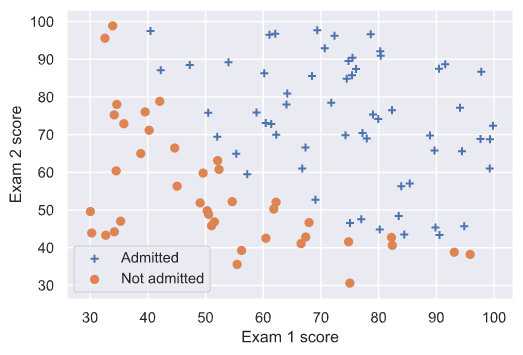
\includegraphics[scale=0.6]{scatter.png}
  \caption{Scatter plot of training data}
  \label{fig:scatter}
\end{figure}

\subsection{Implementation}

\subsubsection{Initializing parameters}

Start by making the parameter array. Remember that the arrays should be rank-2 arrays (have a shape of (m,1)) rather than rank-1 arrays (have a shape of (m,)). For multiple variables problem, remember to scale the feature, that is, the $X$. We will scale the $X$ and store them in $X_scaled$ to be used for \texttt{gradientDescent}.

\begin{lstlisting}{language=Python}
  m, n = X.shape
  ones = np.ones((m,1))
  
  X_scaled = (X - np.mean(X))/np.std(X)
  
  X = np.hstack((ones, X)) # (X, y)) will be used for optimization using scipy.optimize's minimize
  theta = np.zeros((n+1,1))
  y = y[:,np.newaxis]
  
  # for optimization using gradientDescent, we should use scaled X
  X_scaled = np.hstack((ones, X_scaled)) # (X_scaled, y) will be used for optimization gradientDescent
\end{lstlisting}


\subsubsection{Sigmoid function}
Before you start with the actual cost function, recall that the logistic regression hypothesis is defined as:

\begin{align} \label{eq:hx}
  h_\theta(x) = g(\theta^Tx),
\end{align}

where function g is the sigmoid function. The sigmoid function is defined as:

\begin{align} \label{eq:gz}
  g(z) = \frac{1}{1+e^{-z}}
\end{align}

For large positive values of x, the sigmoid should be close to 1, while for large negative values, the sigmoid should be close to 0. Evaluating \texttt{sigmoid(0)} should give you exactly 0.5. Your code should also work with vectors and matrices.

\begin{lstlisting}[language=Python]
  def sigmoid(x):
    return 1/(1+np.exp(-x))
\end{lstlisting}

\subsubsection{Cost function and gradient}

Now you will implement the cost function and gradient for logistic regression. Recall that the cost function in logistic regression is

\begin{align}
  J(\theta) & = \frac{1}{m}\sum_{i=1}^m{\big[-y^{(i)}log(h_\theta(x^{(i)}))-(1-y^{(i)}log(1-h_\theta(x^{(i)})))\big]}
\end{align}

which can be written as \texttt{costFunction}:

\begin{lstlisting}[language=Python]
  def costFunction(theta, X, y):
    m = len(y)
    z = np.dot(X, theta)
    h = sigmoid(z)
    term1 = -y*np.log(h)
    term2 = (1-y)*np.log(1-h)
    cost = np.sum(term1 - term2)/m
    return cost
\end{lstlisting}

The gradient of the cost is a vector of the same length as $\theta$ where the $j^{th}$ element (for $j = 0, 1, ... , n$) is defined as follows:

\begin{align}
  \frac{\partial J(\theta)}{\partial \theta_j} = \frac{1}{m}\sum_{i=1}^m{(h_\theta(x^{(i)})-y^{(i)})\cdot x_j^{(i)}}
\end{align}

which can be written as \texttt{grad}:

\begin{lstlisting}[language=Python]
  def grad(theta, X, y):
  m = len(y)
  h = sigmoid(np.dot(X, theta))
  grad = np.dot(X.T, h-y)/m
  return grad
\end{lstlisting}

Note that while this gradient looks identical to the linear regression gradient, the formula is actually different because linear and logistic regression have different definitions of $h_\theta(x)$. Using the initial parameters of $\theta$, you should see that the cost is about \texttt{0.693}.

There are two ways to optimize the learning parameters: using gradient descent and \verb|minimize| from Scipy's Optimize module. The \texttt{costFunction} and \texttt{grad} function will be used in both technique.


\subsection{Learning parameters}

\subsubsection{Learning parameters using \texttt{gradientDescent}} \label{section:grad}

The code for \texttt{gradientDescent} is based on the following equation:

\begin{align}
  \theta_j  := \theta_j - \alpha\sum_{i=1}^m{(h_\theta(x^{(i)})-y^{(i)})}\cdot x_j^{(i)}
\end{align}

The \texttt{gradientDescent} will return the value of optimized $\theta$ and the $J(\theta)$ after each iteration.

\begin{lstlisting}[language=Python]
  def gradientDescent(X, y, theta_initial, alpha, iterations):
  ''' check "2 Linear regression with one variable"
  page 36
  '''
  m = len(y)
  theta = theta_initial.copy()
  J_val = []
  for i in range(iterations):
      grad2 = grad(theta,X,y)
      cost = costFunction(theta,X,y)
      theta -= alpha*grad2
      J_val.append(cost)
  return theta, J_val
\end{lstlisting}

To determine the $\alpha$ value, we can try several values and plot the computed cost after each iteration. 

\begin{lstlisting}[language=Python]
  iterations = 400
  alpha = [0.01, 0.1, 1]
  theta_optimized1 = 0
  for i in alpha:
      theta_optimized1, J_value =  gradientDescent(X_scaled, y, theta, alpha=i, iterations=iterations)
      plt.plot(np.arange(1,iterations+1), J_value, label='alpha = '+str(i))
  print(f'Optimized theta from gradient descent: {theta_optimized1}')
\end{lstlisting}

From Figure~\ref{fig:gradientdescent}, we will choose \texttt{alpha} of 1 where the cost ($J_\theta$) is decreasing more rapidly. The optimized $\theta$ is: \texttt{1.65947664}, \texttt{3.8670477}, and \texttt{3.60347302}. 

\begin{figure}[h!]
  \centering
  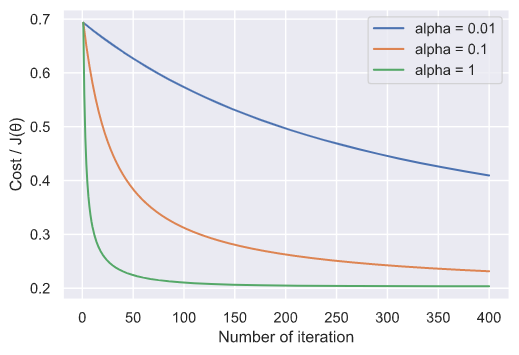
\includegraphics[scale=0.6]{gradientdescent.png}
  \caption{Cost for each iteration for different $\alpha$}
  \label{fig:gradientdescent}
\end{figure}

When we compute the cost using the optimized $\theta$, we will get a lower value of \texttt{0.2036}.

\subsubsection{Learning parameters using \texttt{minimize}} \label{chap:min}

In section~\ref{section:grad} you write a cost function and calculate its gradient, then took a gradient descent step accordingly. This time, instead of taking gradient descent steps, you will use a function in Python's \texttt{optimize}\footnote{More details on Scipy optimize module \href{https://docs.scipy.org/doc/scipy/reference/optimize.html}{here}.} module which is the equivalent of \texttt{fminunc} in Octave/MATLAB.

Octave/MATLAB's \texttt{fminunc} is an optimization solver that finds the minimum of an unconstrained\footnote{Constraints in optimization often refer to constraints on the parameters, for example, constrains that bound the possible values $\theta$ can take (e.g., $\theta\leq 1$). Logistic regression does not have such constraints since $\theta$ is allowed to take any real value.} function. The \texttt{minimize}\footnote{More details on Scipy minimize \href{https://docs.scipy.org/doc/scipy/reference/generated/scipy.optimize.minimize.html#scipy-optimize-minimize}{here}.} from Scipy's library also can do unconstrained minimization of a function and here we will use the Newton-CG method. For logistic regression, you want to optimize the cost function $J(\theta)$ with parameters $\theta$. 

Using \texttt{minimize} we do not need to write any loops ourselves, or set the initial learning rate value like we do for \texttt{alpha} in \texttt{gradientDescent}. You are going to use \texttt{minimize} to find the best parameters $\theta$ for the logistic regression cost function, given a fixed dataset (of $X$ and $y$ values). You will pass to \texttt{minimize} the following inputs:

\begin{enumerate}
  \item The method we are using, \texttt{Newton-CG}
  \item The initial values of the parameters we are trying to optimize.
  \item Objective funtion to be minimized \label{fun}
  \item Gradient of the function that we minimize \label{jac}
  \item Extra arguments passed to two functions in point \ref{fun} and \ref{jac}
\end{enumerate}


\begin{lstlisting}{language=Python}
  from scipy.optimize import minimize
  minimizef = minimize(fun=costFunction, x0=theta.flatten(), jac=grad, args=(X, y.flatten()), method='Newton-CG')
  theta_optimized2 = minimizef.x
\end{lstlisting}

The optimized $\theta$ is: \texttt{-25.16155593}, \texttt{0.20623349}, and \texttt{0.2014734}.

\subsubsection{Evaluating logistic regression} \label{chap:eval}

After learning the parameters, you can use the model to predict whether a particular student will be admitted. For a student with an Exam 1 score of 45 and an Exam 2 score of 85, you should expect to see an admission probability of \texttt{0.776}.

\begin{lstlisting}[language=Python]
  examsval = [[45, 85]]
  m = len(examsval)
  ones = np.ones((m,1))
  x = np.array(examsval)
  x = np.hstack((ones, x)).reshape(m,3)
  pred = sigmoid(np.dot(x, theta_optimized2))
  print(pred)
\end{lstlisting}

Another way to evaluate the quality of the parameters we have found is to see how well learned model predicts on our training set. In logistic regression, the threshold is at $0.5$, thus when we put the value from training dataset and the optimized $\theta$ to equation \ref{eq:hx} and \ref{eq:gz}, all the values more than or equal to $0.5$ will be classified as 'Admitted', or $y=1$.

\begin{lstlisting}[language=Python]
  pred1 = [sigmoid(np.dot(X_scaled, theta_optimized1.flatten())) >= 0.5]
  print(f'Train accuracy using gradientDescent: {np.mean(pred1 == y.flatten()) * 100:.4f}%')
  pred2 = [sigmoid(np.dot(X, theta_optimized2.flatten())) >= 0.5]
  print(f'Train accuracy using minimize: {np.mean(pred2 == y.flatten()) * 100:.4f}%')
\end{lstlisting}

Both method give accuracy of \texttt{89.0000}\%.

\subsection{Plotting the decision boundary}

The decision boundary in this example is linear and the result of optimization using Scipy's \texttt{minimize} can be plotted as follows:

\begin{lstlisting}[language=Python]
  pos = y[:,0] ==1
  neg = y[:,0] ==0
  plt.scatter(X[:,1][pos], X[:,2][pos], marker='+', label='Admitted')
  plt.scatter(X[:,1][neg], X[:,2][neg], label='Not admitted')
    
  x2_value= np.array([np.min(X[:,1]),np.max(X[:,1])])
  y2_value=-(theta_optimized2[0] + theta_optimized2[1]*x2_value)/theta_optimized2[2]
  plt.plot(x2_value,y2_value, 'g', label='scipy "minimize" optimized')
\end{lstlisting}

\begin{figure}[h!]
  \centering
  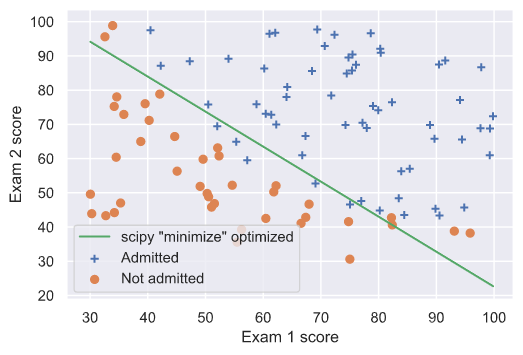
\includegraphics[scale=0.6]{bestfit1.png}
  \caption{Training data with decision boundary from Scipy's \texttt{minimize}}
  \label{fig:bestfit1}
\end{figure}

You can plot the decision boundary obtained from \texttt{gradientDescent} with the same code on \verb|X_scaled|, which will result Figure~\ref{fig:bestfit2}.


\begin{figure}[h!]
  \centering
  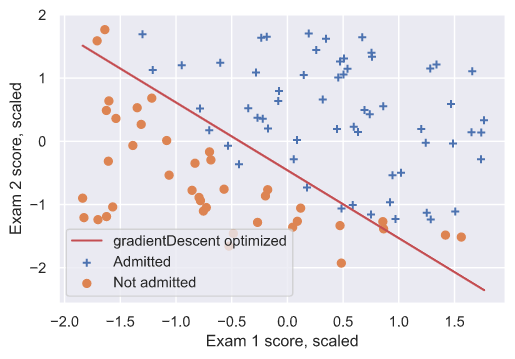
\includegraphics[scale=0.6]{bestfit2.png}
  \caption{Training data with decision boundary from \texttt{gradientDescent}}
  \label{fig:bestfit2}
\end{figure}

\hrulefill

\section{Regularized logistic regression}

In this part of the exercise, you will implement regularized logistic regression to predict whether microchips from a fabrication plant passes quality assurance (QA). During QA, each microchip goes through various tests to ensure it is functioning correctly.

Suppose you are the product manager of the factory and you have the test results for some microchips on two different tests. From these two tests, you would like to determine whether the microchips should be accepted or rejected. To help you make the decision, you have a dataset of test results on past microchips, from which you can build a logistic regression model. This guide and the framework code in \texttt{exercise2-2.ipynb} will guide you through the exercise.

\subsection{Visualizing the data}

Similar to the previous parts of this exercise, we plot the data to generate a figure like Figure~\ref{fig:scatter1}, where the axes are the two test scores, and the positive ($y = 1$, accepted) and negative ($y = 0$, rejected) examples are shown with different markers.

\begin{figure}[h!]
  \centering
  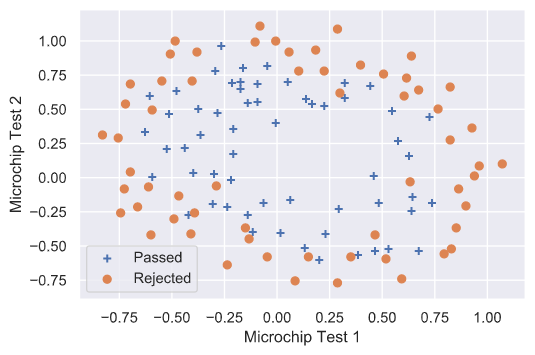
\includegraphics[scale=0.6]{scatter1.png}
  \caption{Plot of training data}
  \label{fig:scatter1}
\end{figure}

Figure~\ref{fig:scatter1} shows that our dataset cannot be separated into positive and negative examples by a straight-line through the plot. Therefore, a straightforward application of logistic regression will not perform well on this dataset since logistic regression will only be able to find a linear decision boundary.


\subsection{Feature mapping}

One way to fit the data better is to create more features from each data point. In the \texttt{mapFeature}, we will map the features into all polynomial terms of $x_1$ and $x_2$ up to the sixth power.

\begin{align}
  \mathbf mapFeature(x) = \begin{bmatrix} 1 \\ x_1 \\ x_2 \\ x_1^2 \\ x_1x_2 \\ x_2^2 \\ x_1^3 \\ \vdots \\ x_1x_2^5 \\ x_2^6 \end{bmatrix}
\end{align}

As a result of this mapping, our vector of two features (the scores on two QA tests) has been transformed into a 28-dimensional vector. A logistic regression classifier trained on this higher-dimension feature vector will have
a more complex decision boundary and will appear nonlinear when drawn in our 2-dimensional plot.

While the feature mapping allows us to build a more expressive classifier, it also more susceptible to overfitting. In the next parts of the exercise, you will implement regularized logistic regression to fit the data and also see for yourself how regularization can help combat the overfitting problem.


\subsection{Cost function and gradient} \label{val:costawal}

Now you will implement code to compute the cost function and gradient for regularized logistic regression. Make a function to compute the cost (\texttt{costFunctionReg}) and gradient (\texttt{grad}). 

Recall that the regularized cost function in logistic regression is

\begin{align}
  J(\theta) = \frac{1}{m}\sum_{i=1}^m{\big[-y^{(i)}log(h_\theta(x^{(i)}))-(1-y^{(i)}log(1-h_\theta(x^{(i)})))\big]} + \frac{\lambda}{2m}\sum_{j=1}^n{\theta_j^2}
\end{align}

\begin{lstlisting}[language=Python]
  def costFunctionReg(theta, X, y, lmbd):
  m = len(y)
  z = np.dot(X, theta)
  term1 = -y*np.log(sigmoid(z))
  term2 = (1-y)*np.log(1-sigmoid(z))
  J = (1/m)*np.sum(term1 - term2) + lmbd/(2*m)*np.sum(theta**2)
  return J
\end{lstlisting}

The gradient of the cost function is a vector where the $j^{th}$ element is defined as follows:

\begin{align}
  \frac{\partial J(\theta)}{\partial \theta_0} & = \frac{1}{m}\sum_{i=1}^m{(h_\theta(x^{(i)})-y^{(i)}) x_j^{(i)}} & \text{for} j & = 0 \\
  \frac{\partial J(\theta)}{\partial \theta_j} & = \bigg(\frac{1}{m}\sum_{i=1}^m{(h_\theta(x^{(i)})-y^{(i)}) x_j^{(i)}}\bigg) + \frac{\lambda}{m}\theta_j & \text{for} j & \geq 0
\end{align}

\begin{lstlisting}[language=Python]
  def grad(theta, X, y, lmbd):
  m = len(y)
  h = sigmoid(np.dot(X,theta))
  grad = (1/m)*np.dot(X.T, h-y)
  return grad + (lmbd/m)*theta
\end{lstlisting}

Using \texttt{lmbd}($\lambda$) of 1, the cost is about \texttt{0.693}.

\subsection{Learning parameters}

\subsubsection{Learning parameters using \texttt{gradientDescent}} 

The code for \texttt{gradientDescent} is based on the following equation:

\begin{align}
  \theta_j := \theta_j - \alpha \bigg(\frac{1}{m}\sum_{i=1}^m{(h_\theta(x^{(i)})-y^{(i)}) x_j^{(i)}} + \frac{\lambda}{m}\theta_j\bigg)
  \end{align}

The \texttt{gradientDescent} wiill return the value of optimized $\theta$ and the $J(\theta)$ after each iteration. 

\begin{lstlisting}[language=Python]
  def gradientDescent(X, y, theta_initial, alpha, iterations, lmbd):
  m = len(y)
  theta = theta_initial.copy()
  J_val = []
  for i in range(iterations):
      grad2 = grad(theta, X, y, lmbd)
      cost = costFunctionReg(theta, X, y, lmbd)
      theta -= alpha*grad2
      J_val.append(cost)
  return theta, J_val
\end{lstlisting}

We can determine the $\alpha$ and $\lambda$ value through iterations and plot the computed cost after each iteration. For example, here we try \texttt{alpha} value of \texttt{0.01}, \texttt{0.03}, \texttt{0.1}, \texttt{0.3}, and \texttt{1}. Using similar code to search for $\lambda$ value we wil get Figure~\ref{fig:gradlambda}. 

\begin{lstlisting}[language=Python]
  iterations = 800
  alpha = [0.01, 0.03, 0.1, 0.3, 1]
  theta_optimized1 = 0
  for i in alpha:
      theta_optimized1, J_value =  gradientDescent(X_mapped, y, theta, alpha=i, iterations=iterations, lmbd=1)
      plt.plot(np.arange(1,iterations+1), J_value, label='alpha = '+str(i))
\end{lstlisting}

\begin{figure}[h!]
  \centering
  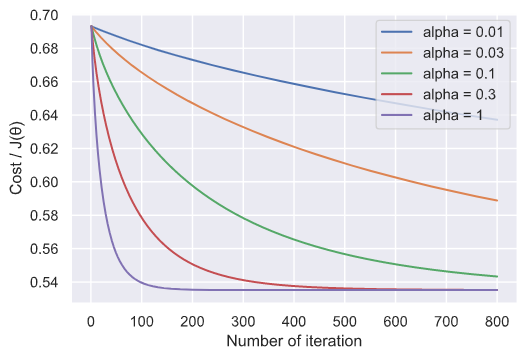
\includegraphics[scale=0.6]{gradientdescentalpha.png}
  \caption{Cost for each iteration for different $\alpha$}
  \label{fig:gradalpha}
\end{figure}

\begin{figure}[h!]
  \centering
  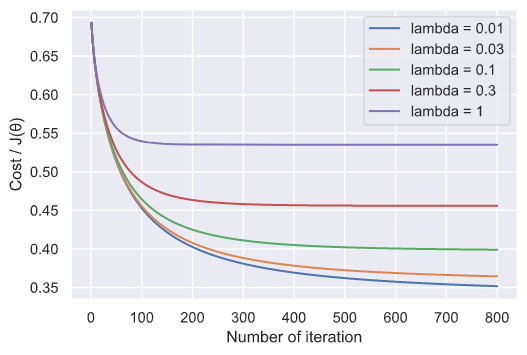
\includegraphics[scale=0.6]{gradientdescentlambda.png}
  \caption{Cost for each iteration for different $\lambda$}
  \label{fig:gradlambda}
\end{figure}

From Figure~\ref{fig:gradalpha}, $\alpha = 1$ gives the steepest decrease of the cost. From Figure~\ref{fig:gradlambda}, we will choose \texttt{lmbd} of 0.03 where the cost ($J_\theta$) is decreasing more rapidly. The \texttt{gradientDescent} returns the optimized $\theta$ value which has $28$ elements. 

Using the optimized \texttt{alpha} and \texttt{lmbd}, we can compute the optimized $\theta$ and plot the cost function as follows:

\begin{lstlisting}[language=Python]
  theta_optimized1, J_value =  gradientDescent(X_mapped, y, theta, alpha=1, iterations=iterations, lmbd=0.03)
  plt.plot(np.arange(1,iterations+1), J_value)
\end{lstlisting}

\begin{figure}[h!]
  \centering
  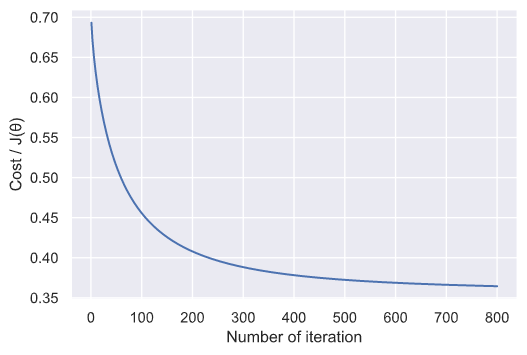
\includegraphics[scale=0.6]{gradientdescent2.png}
  \caption{Cost for each iteration}
  \label{fig:graddescent2}
\end{figure}

The cost is computed using \texttt{costFunctionReg}, \verb|theta_optimized1| and $\lambda = 0.03$, which gives value of \texttt{0.3644891}, lower than when the $\theta$ was 0, which was \texttt{0.693} in Section~\ref{val:costawal}.



\begin{lstlisting}[language=Python]
  J_optimized1 = costFunctionReg(theta_optimized1, X_mapped, y, lmbd=0.03)
\end{lstlisting}

\subsubsection{Learning parameters using \texttt{minimize}}

Much like optimizing $\theta$ in Section~\ref{chap:min}, you will use \texttt{minimize} function from Scipy's \texttt{optimize} module. The only difference with the code in Section~\ref{chap:min} is we need the value of $\lambda$ for the regularization parameter. 

\begin{lstlisting}[language=Python]
  from scipy.optimize import minimize
  lmbd = 0.03
  temp = minimize(fun = costFunctionReg, 
                      x0 = theta.flatten(),jac = grad, 
                      args = (X_mapped, y.flatten(), lmbd), 
                      method='Newton-CG')
  theta_optimized2 = temp.x
\end{lstlisting}

The cost is computed using \texttt{costFunctionReg}, \verb|theta_optimized2| and $\lambda = 0.03$, which gives value of \texttt{0.356175}, lower than when the $\theta$ was 0, which was \texttt{0.693}in Section~\ref{val:costawal}.

\subsection{Plotting the decision boundary}

\subsubsection{Comparing \texttt{gradientDescent} and \texttt{minimize}}

To visualize the model learned by this classifier, we plot the (non-linear) decision boundary that separates the positive and negative examples by computing the classifier’s predictions on an evenly spaced grid and then and drew a contour plot of where the predictions change from y = 0 to y = 1. We write a function called \texttt{mapFeaturePlot} to help map the features. 

\begin{lstlisting}[language=Python]
  def mapFeaturePlot(X1, X2, degree):
  out = np.ones(1)
  for i in range(1,degree+1):
      for j in range(i+1):
          feature = (X1**(i-j) * X2**j)
          out = np.hstack((out,feature))
  return out
\end{lstlisting}

The code below is plotting the decision boundary with $\theta$ obtained from \texttt{gradientDescent} (\verb|theta_optimized1|) and from \texttt{minimize} (\verb|theta_optimized2|). The result is in Figure~\ref{fig:bound003}. 

\begin{lstlisting}[language=Python]
  u_vals = np.linspace(-1,1.5,50)
  v_vals= np.linspace(-1,1.5,50)
  z1=np.zeros((len(u_vals),len(v_vals)))
  z2=np.zeros((len(u_vals),len(v_vals)))
  
  for i in range(len(u_vals)):
      for j in range(len(v_vals)):
          z1[i,j] = np.dot(mapFeaturePlot(u_vals[i],v_vals[j],6), theta_optimized1)
  
  for i in range(len(u_vals)):
      for j in range(len(v_vals)):
          z2[i,j] = np.dot(mapFeaturePlot(u_vals[i],v_vals[j],6), theta_optimized2.reshape(len(theta_optimized2),1))
  
  plt.contour(u_vals,v_vals,z1.T,0, colors='g', label='gradientDescent')
  plt.contour(u_vals,v_vals,z2.T,0, colors='r', label='minimize')
  
  plt.xlabel('Microchip Test 1')
  plt.ylabel('Microchip Test 2')
\end{lstlisting}

\begin{figure}[h!]
  \centering
  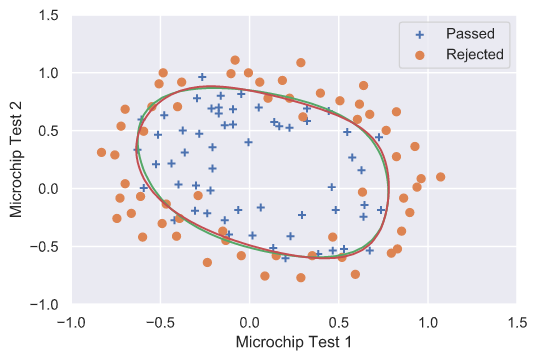
\includegraphics[scale=0.6]{bound003.png}
  \caption{Training data with decision boundary ($\lambda = 1$)}
  \label{fig:bound003}
\end{figure}

The green line is the boundary line of \texttt{gradientDescent} method, while the red line is the boundary line of \texttt{minimize}. As seen in Figure~\ref{fig:bound003}, the two methods have similar boundary line. We can evaluate our methods by calculating the training accuracy as we did in Section~\ref{chap:eval}. Below is the code to check the training accuracy:

\begin{lstlisting}[language=Python]
  pred1 = [sigmoid(np.dot(X_mapped, theta_optimized1.flatten())) >= 0.5]
  print(f'Train accuracy using gradientDescent: {np.mean(pred1 == y.flatten()) * 100:.4f}%')
  pred2 = [sigmoid(np.dot(X_mapped, theta_optimized2)) >= 0.5]
  print(f'Train accuracy using fmin_tnc: {np.mean(pred2 == y.flatten()) * 100:.4f}%')
\end{lstlisting}

\texttt{minimize} method has a slightly higher training accuracy, \texttt{84.7458}\%, compared to that of \texttt{gradientDescent} which is only \texttt{83.8983}\%.

We can try out different regularization parameters ($\lambda$) for the dataset to understand how regularization prevents overfitting. Notice the changes in the decision boundary as you vary $\lambda$. With a small $\lambda$, you should find that the classifier gets almost every training example correct, but draws a very complicated boundary, thus overfitting the data (Figure~\ref{fig:bound0}). 

With a larger $\lambda$, you should see a plot that shows an simpler decision boundary which still separates the positives and negatives fairly well. However, if $\lambda$ is set to too high a value, you will not get a good fit and the decision boundary will not follow the data so well, thus underfitting the data (Figure~\ref{fig:bound10}).

\begin{figure}[h!]
  \centering
  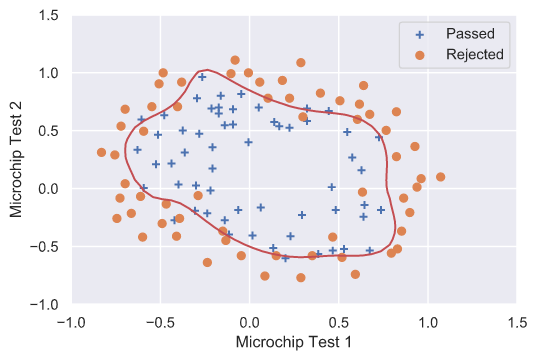
\includegraphics[scale=0.6]{bound0.png}
  \caption{No regularization (Overfitting) ($\lambda=0$)}
  \label{fig:bound0}
\end{figure}

\begin{figure}[h!]
  \centering
  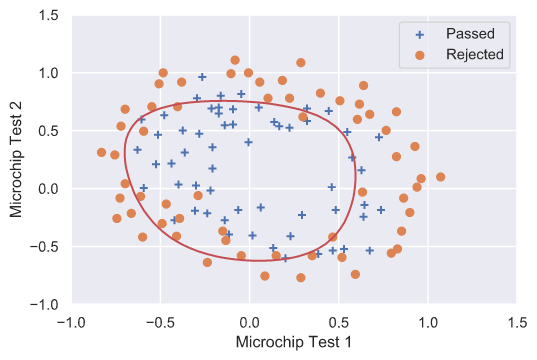
\includegraphics[scale=0.6]{bound10.png}
  \caption{Too much regularization (Underfitting) ($\lambda=100$)}
  \label{fig:bound10}
\end{figure}


\end{document}
